%%%%%%%%%%%%%%%%%%%%%%%%%%%%%%%%%%%%%%%%%
% Lachaise Assignment
% LaTeX Template
% Version 1.0 (26/6/2018)
%
% This template originates from:
% http://www.LaTeXTemplates.com
%
% Authors:
% Marion Lachaise & François Févotte
% Vel (vel@LaTeXTemplates.com)
%
% License:
% CC BY-NC-SA 3.0 (http://creativecommons.org/licenses/by-nc-sa/3.0/)
% 
%%%%%%%%%%%%%%%%%%%%%%%%%%%%%%%%%%%%%%%%%

%----------------------------------------------------------------------------------------
%	PACKAGES AND OTHER DOCUMENT CONFIGURATIONS
%----------------------------------------------------------------------------------------

\documentclass{article}

%%%%%%%%%%%%%%%%%%%%%%%%%%%%%%%%%%%%%%%%%
% Lachaise Assignment
% Structure Specification File
% Version 1.0 (26/6/2018)
%
% This template originates from:
% http://www.LaTeXTemplates.com
%
% Authors:
% Marion Lachaise & François Févotte
% Vel (vel@LaTeXTemplates.com)
%
% License:
% CC BY-NC-SA 3.0 (http://creativecommons.org/licenses/by-nc-sa/3.0/)
% 
%%%%%%%%%%%%%%%%%%%%%%%%%%%%%%%%%%%%%%%%%

%----------------------------------------------------------------------------------------
%	PACKAGES AND OTHER DOCUMENT CONFIGURATIONS
%----------------------------------------------------------------------------------------

\usepackage{amsmath,amsfonts,stmaryrd,amssymb} % Math packages

\usepackage{enumerate} % Custom item numbers for enumerations

\usepackage[ruled]{algorithm2e} % Algorithms

\usepackage[framemethod=tikz]{mdframed} % Allows defining custom boxed/framed environments

\usepackage{listings}
\usepackage{color}

\definecolor{dkgreen}{rgb}{0,0.6,0}
\definecolor{gray}{rgb}{0.5,0.5,0.5}
\definecolor{mauve}{rgb}{0.58,0,0.82}

\lstset{
    language=C,
    aboveskip=3mm,
    belowskip=3mm,
    showstringspaces=false,
    columns=flexible,
    basicstyle={\small\ttfamily},
    numbers=none,
    numberstyle=\tiny\color{gray},
    keywordstyle=\color{blue},
    commentstyle=\color{dkgreen},
    stringstyle=\color{mauve},
    breaklines=true,
    breakatwhitespace=true,
    tabsize=4
}

%----------------------------------------------------------------------------------------
%	DOCUMENT MARGINS
%----------------------------------------------------------------------------------------

\usepackage{geometry} % Required for adjusting page dimensions and margins

\geometry{
	paper=a4paper, % Paper size, change to letterpaper for US letter size
	top=2.5cm, % Top margin
	bottom=3cm, % Bottom margin
	left=2.5cm, % Left margin
	right=2.5cm, % Right margin
	headheight=14pt, % Header height
	footskip=1.5cm, % Space from the bottom margin to the baseline of the footer
	headsep=1.2cm, % Space from the top margin to the baseline of the header
	%showframe, % Uncomment to show how the type block is set on the page
}

%----------------------------------------------------------------------------------------
%	FONTS
%----------------------------------------------------------------------------------------

\usepackage[utf8]{inputenc} % Required for inputting international characters
\usepackage[T1]{fontenc} % Output font encoding for international characters

\usepackage{XCharter} % Use the XCharter fonts
\usepackage{microtype} 

%----------------------------------------------------------------------------------------
%	COMMAND LINE ENVIRONMENT
%----------------------------------------------------------------------------------------

% Usage:
% \begin{commandline}
%	\begin{verbatim}
%		$ ls
%		
%		Applications	Desktop	...
%	\end{verbatim}
% \end{commandline}

\mdfdefinestyle{commandline}{
	leftmargin=10pt,
	rightmargin=10pt,
	innerleftmargin=15pt,
	middlelinecolor=black!50!white,
	middlelinewidth=2pt,
	frametitlerule=false,
	backgroundcolor=black!5!white,
	frametitle={Command Line},
	frametitlefont={\normalfont\sffamily\color{white}\hspace{-1em}},
	frametitlebackgroundcolor=black!50!white,
	nobreak,
}

% Define a custom environment for command-line snapshots
\newenvironment{commandline}{
	\medskip
	\begin{mdframed}[style=commandline]
}{
	\end{mdframed}
	\medskip
}

%----------------------------------------------------------------------------------------
%	FILE CONTENTS ENVIRONMENT
%----------------------------------------------------------------------------------------

% Usage:
% \begin{file}[optional filename, defaults to "File"]
%	File contents, for example, with a listings environment
% \end{file}

\mdfdefinestyle{file}{
	innertopmargin=1.6\baselineskip,
	innerbottommargin=0.8\baselineskip,
	topline=false, bottomline=false,
	leftline=false, rightline=false,
	leftmargin=2cm,
	rightmargin=2cm,
	singleextra={%
		\draw[fill=black!10!white](P)++(0,-1.2em)rectangle(P-|O);
		\node[anchor=north west]
		at(P-|O){\ttfamily\mdfilename};
		%
		\def\l{3em}
		\draw(O-|P)++(-\l,0)--++(\l,\l)--(P)--(P-|O)--(O)--cycle;
		\draw(O-|P)++(-\l,0)--++(0,\l)--++(\l,0);
	},
	nobreak,
}

% Define a custom environment for file contents
\newenvironment{file}[1][File]{ % Set the default filename to "File"
	\medskip
	\newcommand{\mdfilename}{#1}
	\begin{mdframed}[style=file]
}{
	\end{mdframed}
	\medskip
}

%----------------------------------------------------------------------------------------
%	NUMBERED QUESTIONS ENVIRONMENT
%----------------------------------------------------------------------------------------

% Usage:
% \begin{question}[optional title]
%	Question contents
% \end{question}

\mdfdefinestyle{question}{
	innertopmargin=1.2\baselineskip,
	innerbottommargin=0.8\baselineskip,
	roundcorner=5pt,
	nobreak,
	singleextra={%
		\draw(P-|O)node[xshift=1em,anchor=west,fill=white,draw,rounded corners=5pt]{%
		Example \theQuestion\questionTitle};
	},
}

\newcounter{Question} % Stores the current question number that gets iterated with each new question

% Define a custom environment for numbered questions
\newenvironment{question}[1][\unskip]{
	\bigskip
	\stepcounter{Question}
	\newcommand{\questionTitle}{~#1}
	\begin{mdframed}[style=question]
}{
	\end{mdframed}
	\medskip
}

%----------------------------------------------------------------------------------------
%	WARNING TEXT ENVIRONMENT
%----------------------------------------------------------------------------------------

% Usage:
% \begin{warn}[optional title, defaults to "Warning:"]
%	Contents
% \end{warn}

\mdfdefinestyle{warning}{
	topline=false, bottomline=false,
	leftline=false, rightline=false,
	nobreak,
	singleextra={%
		\draw(P-|O)++(-0.5em,0)node(tmp1){};
		\draw(P-|O)++(0.5em,0)node(tmp2){};
		\fill[black,rotate around={45:(P-|O)}](tmp1)rectangle(tmp2);
		\node at(P-|O){\color{white}\scriptsize\bf !};
		\draw[very thick](P-|O)++(0,-1em)--(O);%--(O-|P);
	}
}

% Define a custom environment for warning text
\newenvironment{warn}[1][Warning:]{ % Set the default warning to "Warning:"
	\medskip
	\begin{mdframed}[style=warning]
		\noindent{\textbf{#1}}
}{
	\end{mdframed}
}

%----------------------------------------------------------------------------------------
%	INFORMATION ENVIRONMENT
%----------------------------------------------------------------------------------------

% Usage:
% \begin{info}[optional title, defaults to "Info:"]
% 	contents
% 	\end{info}

\mdfdefinestyle{info}{%
	topline=false, bottomline=false,
	leftline=false, rightline=false,
	nobreak,
	singleextra={%
		\fill[black](P-|O)circle[radius=0.4em];
		\node at(P-|O){\color{white}\scriptsize\bf i};
		\draw[very thick](P-|O)++(0,-0.8em)--(O);%--(O-|P);
	}
}

% Define a custom environment for information
\newenvironment{info}[1][Info:]{ % Set the default title to "Info:"
	\medskip
	\begin{mdframed}[style=info]
		\noindent{\textbf{#1}}
}{
	\end{mdframed}
}

\usepackage{siunitx}
\usepackage[hidelinks]{hyperref} % Include the file specifying the document structure and custom commands
\usepackage{graphicx}
\usepackage{siunitx}
\newcommand{\tmk}{\texttt{taamak.h}}

%----------------------------------------------------------------------------------------
%	ASSIGNMENT INFORMATION
%----------------------------------------------------------------------------------------

\title{\tmk{} Documentation} % Title of the assignment

\author{Zeyuan Fang\\ \texttt{fang.zeyuan@outlook.com}} % Author name and email address

\date{v1.0.0-rc} % University, school and/or department name(s) and a date

%----------------------------------------------------------------------------------------
\setcounter{secnumdepth}{0}
\setlength{\parindent}{0pt}

\begin{document}

\maketitle % Print the title
\tableofcontents

%----------------------------------------------------------------------------------------
%	INTRODUCTION
%----------------------------------------------------------------------------------------
\section{Introduction}
\tmk{} is a free/open-source C library for calculating responses in a truncated multi-layer linear-elastic pavement system. Its features include:
\begin{itemize}
    \item Evaluation of stresses and displacements in a trimmed homogeneous linear elastic pavement model, subject to a square patch stress.
    \item Evaluation of surface deflection on a truncated multi-layered linear elastic pavement model, subject to a square patch stress.
    \item Back-calculation of Effective Slope Angle (ESA) of a homogeneous/multi-layered linear elastic pavement model, utilising FWD deflection measurements tested near the edge/discontinuity of the pavement system.
\end{itemize}
\begin{info} % ESA
    Effective Slope Angle (ESA) is a novel entity in pavement engineering that quantifies the lateral support provided to the pavement system by the omitted region. For the scenario where a pavement system is abutting with a local soil medium, ESA represents the side support contributed by the local soil. In the scenario where a pavement system is experiencing significant cracking, ESA characterises the support offered by the intact material or through a stress-transfer mechanism across crack interfaces (or a combination of both). Under ideal conditions, ESA is \ang{0} (representing a half-space model), while the most extreme scenario presents ESA at \ang{90}.
\end{info}

\tmk{} is available on GitHub at https:
//github.com/veslrs/taamak.h. It is distributed under the MIT License; users should note the additional notices and licensing terms for third party dependencies included with the repository. 

\clearpage

\section{\tmk{} Tutorial}
In this tutorial, we illustrate the usage of \tmk{} via two trivial examples.

\subsection{Example 1: Multi-layer near-edge deflections}
As a first example, we'll look at the following simple problem calculating the deflections of a truncated two-layered linear-elastic pavement system, subject to a near edge patch stress.
\begin{figure}[h]
    \centering
    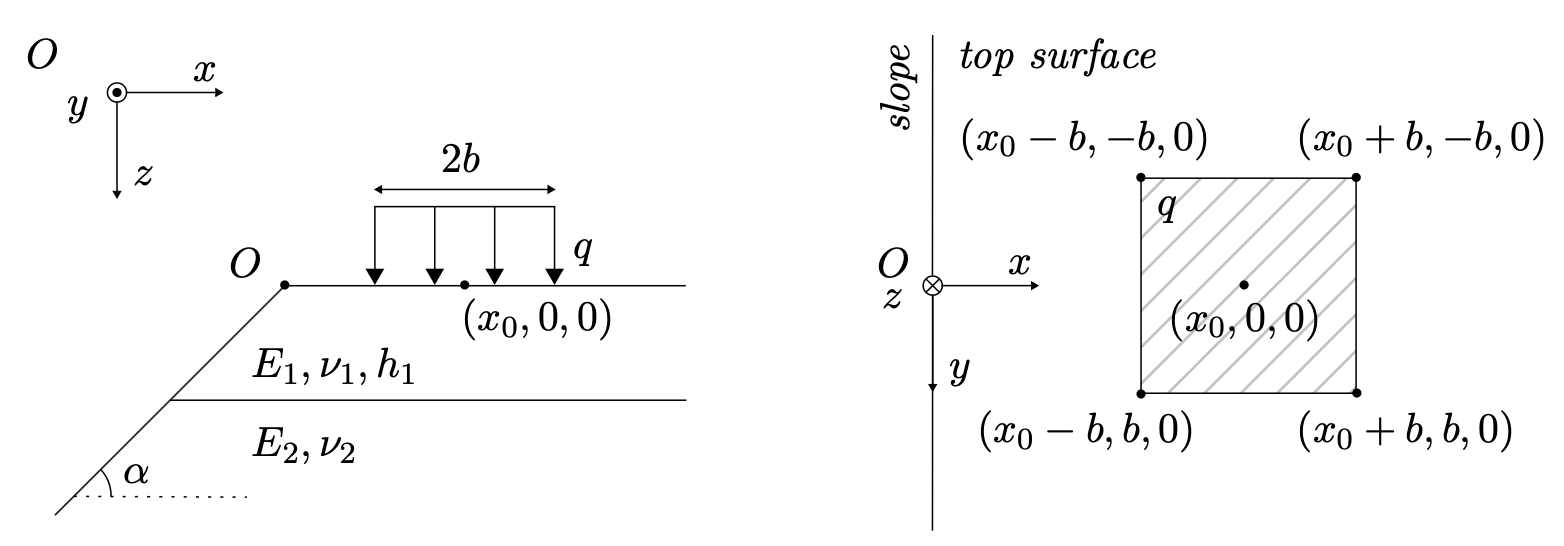
\includegraphics[width=0.7\linewidth]{figures/ex1}
    \label{fig:ex1}
\end{figure}
\begin{question}[\itshape (multi-layer near-edge deflections)]
    Square stress patch of side \( 2b = \SI{300}{\milli\meter} \) with uniform intensity \( q = \SI{0.5}{\mega\pascal} \) is applied to a trimmed two-layered elastic half‑space. The elastic properties of Layer \( i \) \( (i=1,2) \) are Young's modulus \( E_1 = \SI{500}{\mega\pascal}, E_2 = \SI{50}{\mega\pascal} \) and Poisson ratio \( \nu_1 = 0.3, \nu_2 = 0.4 \); the corresponding layer thickness are \( h_1 = \SI{600}{\milli\meter} \), and a semi-infinite \( h_2 \). A Cartesian coordinate system placed at origin \( O \): \( x \)-axis toward the patch, \( y \)-axis along the patch edge, and \( z \)-axis downward. The free side slope has an angle \( \alpha = \ang{75} \) with the top surface. In the top view the patch centroid lies at \( x = x_0 = \SI{300}{\milli\meter}\) and \( y = z = 0 \) with \( x_0 > b \). We are asked to evaluate deflections at four points (in \si{\milli\meter}): \( (0,0,0), (300,0,0), (600,150,0) \text{ and } (1200,300,0) \). 
\end{question}

To implement the above example in C we would first do:
\begin{file}[ex\_01.c]
\begin{lstlisting}[language=C]
#define TMK_IMPLEMENTATION
#include "taamak.h"
\end{lstlisting}
\end{file}
to include the \tmk{} header file as well as enabling the implementation. Then we would define our model object as:
\begin{file}[ex\_01.c]
\begin{lstlisting}[language=C]
tmk_model mdl;
tmk_init(&mdl, 2);
\end{lstlisting}
\end{file}
where the model \texttt{mdl} is initialised with two layers. For the specification of the model, we do:
\begin{file}[ex\_01.c]
\begin{lstlisting}[language=C]
// set loadings
tmk_vec3 center = {300.0, 0.0, 0.0};
double b = 150.0;
double q = 0.5;
tmk_set_load(&mdl, center, b, q);

// set layer compositions
tmk_set_composition(&mdl, (double[]){0.0, 600.0});

// set layer properties
tmk_hs hs[] = {
    // layer #1
    {
        .youngs_modulus = 500.0,
        .poissons_ratio = 0.3,
    },
    // layer #2
    {
        .youngs_modulus = 50.0,
        .poissons_ratio = 0.4,
    },
};
tmk_set_material_properties(&mdl, hs);

// set slope angle
tmk_set_slope_angle(&mdl, 75.0);
\end{lstlisting}
\end{file}

There are two things to notice here. First, the function \texttt{tmk\_set\_composition} takes the depth of the \textit{top interface} of each layer to specify the layer compositions. That does not affect the the application in a two-layered system, but for three layers and above, one should be careful with the calculation of the \textit{top depths} from the given layer thicknesses. Second, one should check manually the alignment of the number of layers ad the number of material properties. 

Now we set up evaluation points:
\begin{file}[ex\_01.c]
\begin{lstlisting}[language=C]
tmk_vec3 pts[] = {
        {0.0, 0.0, 0.0},
        {300.0, 0.0, 0.0},
        {600.0, 150.0, 0.0},
        {1200.0, 300.0, 0.0},
};
tmk_set_evaluation_points(&mdl, 4, pts);
\end{lstlisting}
\end{file}

At this point, we can call \texttt{tmk\_solve} to perform the evaluation, and lastly, we should call \texttt{tmk\_checkout} to return evaluation status:
\begin{file}[ex\_01.c]
\begin{lstlisting}[language=C]
// solve
tmk_solve(&mdl);

// done!
tmk_checkout(&mdl);
\end{lstlisting}
\end{file}

Assuming we save this in a file \texttt{ex\_01.c}, we would compile and link (on Unix) with:
\begin{commandline}
\begin{verbatim}
$ cc ex_01.c -o ex_01 -lopenblas
\end{verbatim}
\end{commandline}

The result of running the program should then be something like:
\begin{commandline}
\begin{verbatim}
x[mm]   y[mm]   deflection[micron]
0       0       651.5
300     0       810.8
600     150     521.0
1200    300     326.9
\end{verbatim}
\end{commandline}

That is, it computed the deflections (in \si{\micro\meter}) of given evaluation points.

\subsection{Example 2: ESA back-calculation}
In the second example, we'll look at the another simple problem back-calculating the Effective Slope Angle (ESA) of a two-layered linear-elastic pavement structure.
\begin{figure}[h]
    \centering
    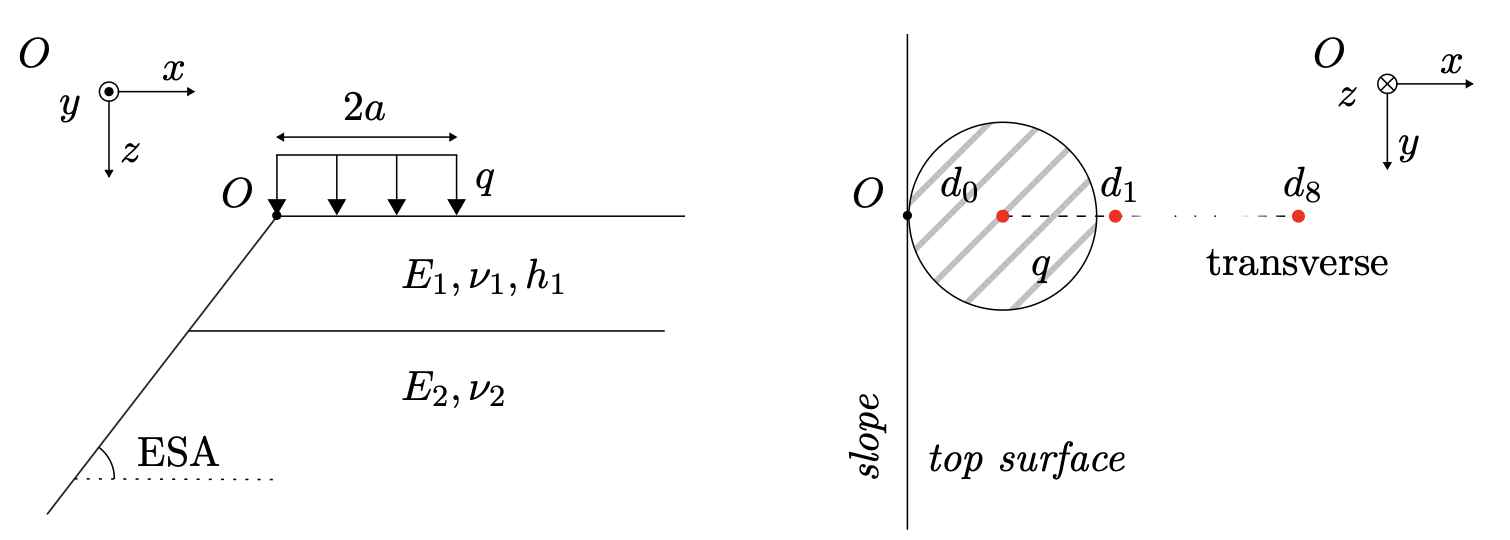
\includegraphics[width=0.7\linewidth]{figures/ex2}
    \label{fig:ex2}
\end{figure}
\begin{question}[\itshape (ESA back-calculation)]
    An FWD load plate with diameter \( 2a = \SI{300}{\milli\meter} \) (simulated by square patch with \( b = \SI{133}{\milli\meter} \) to ensure same distribution area), exerts a uniform vertical stress with intensity \( q = \SI{0.707}{\mega\pascal} \). A two-layered elastic pavement structure. The load plate is placed near an edge of a pavement abutting local soil medium, or near the opening of a wide top-down crack, thus the pavement model was considered to be trimmed with an unknown ESA. A right-handed Cartesian coordinate system is introduced at the origin \( O \), with the \( x \)-axis oriented perpendicular to the edge and pointing away from it, the \( y \)-axis coinciding with the edge, and the \( z \)-axis pointing downward into the medium. The cross-sectional view of the three-layered system. The elastic properties of Layer \( i \) \( (i=1,2) \) are Young's modulus \( E_1 = \SI{500}{\mega\pascal}, E_2 = \SI{80}{\mega\pascal} \) and Poisson ratio \( \nu_1 = 0.3, \nu_2 = 0.4 \); the corresponding layer thickness are \( h_1 = \SI{750}{\milli\meter} \), and a semi-infinite \( h_2 \). The load-plate is tangent to the edge, with the centre of the circle placed at \( x = a \). The red markers, labelled \( d_0, \ldots, d_8 \), represent the sensors (geophones) of the FWD with transverse orientation, with \( x \)-offsets from the centre of the FWD load plate: \( 0, 200, 300, 450, 600, 900, 1200, 1500, \text{ and } \SI{1800}{\milli\meter} \), and the corresponding FWD deflection measurements: \( 0.659, 0.593, 0.404, 0.338, 0.287, 0.253, 0.201, 0.163, 0.134, \text{ and } \SI{0.113}{\milli\meter} \). We are asked to back-calculate the ESA. 
\end{question}

To start with, we include the header file and implementation, then initialise and set up our model with available model specification parameters, same as Example 1:
\begin{file}[ex\_02.c]
\begin{lstlisting}[language=C]
#define TMK_IMPLEMENTATION
#include "taamak.h"

int main(void)
{
    // set loadings
    tmk_vec3 center = {150.0, 0.0, 0.0};
    double b = 133.0;
    double q = 0.707;
    tmk_set_load(&mdl, center, b, q);

    // set layer compositions
    tmk_set_composition(&mdl, (double[]){0.0, 750.0});

    // set layer properties
    tmk_hs hs[] = {
        // layer #1
        {
            .youngs_modulus = 500.0,
            .poissons_ratio = 0.3,
        },
        // layer #2
        {
            .youngs_modulus = 80.0,
            .poissons_ratio = 0.4,
        },
    };
    tmk_set_material_properties(&mdl, hs);
    
    // to be continued ...
    
}
\end{lstlisting}
\end{file}

Note that we do not initialise slope angle: it doesn't exist yet! 

From here the set up diverges from Example 1: we now specify the FWD measurement coordinated and the corresponding data:
\begin{file}[ex\_02.c]
\begin{lstlisting}[language=C]
// set FWD measurement points
int npts = 10;
tmk_vec3 pts[] = {
    {150.0,  0.0, 0.0},
    {250.0,  0.0, 0.0},
    {350.0,  0.0, 0.0},
    {450.0,  0.0, 0.0},
    {600.0,  0.0, 0.0},
    {750.0,  0.0, 0.0},
    {1050.0, 0.0, 0.0},
    {1350.0, 0.0, 0.0},
    {1650.0, 0.0, 0.0},
    {1950.0, 0.0, 0.0},
};
double vals[] = {
    0.659, 0.593, 0.404, 0.338, 0.287, 
    0.253, 0.201, 0.163, 0.134, 0.113,
};
tmk_set_measurement(&mdl, npts, pts, vals);
\end{lstlisting}
\end{file}

Pretty straight-forward. Finally, same as Example 1, we can call \texttt{tmk\_solve} to perform the ESA back-calculation, and call \texttt{tmk\_checkout} to return evaluation status:
\begin{file}[ex\_02.c]
\begin{lstlisting}[language=C]
// solve effective slope angle
tmk_solve(&mdl);

// done!
tmk_checkout(&mdl);
\end{lstlisting}
\end{file}

Assuming we save this in a file \texttt{ex\_02.c}, we would compile and link (on Unix) with:
\begin{commandline}
\begin{verbatim}
$ cc ex_02.c -o ex_02 -lopenblas
\end{verbatim}
\end{commandline}

The result of running the program should then be something like:
\begin{commandline}
\begin{verbatim}
[INFO] Iteration 11: trial algle = 62.2 [deg]. Evaluating......
[INFO]   Signed difference with 62.2 [deg]: 0.000025
[INFO] Equivalent Slope Angle = 62.2 [deg]
\end{verbatim}
\end{commandline}

That is, the remaining lateral support of the pavement structure can be quantified by an ESA = \ang{62.2}.

\clearpage

\section{\tmk{} Reference} 
\tmk{} is a library, not a stand-alone program -- it is designed to be called from your own program in C programming language. This reference section describes the programming interface (API) of \tmk{}. 

% API reference
\subsection{Compile and linking}
An \tmk{} program begins with including the header file. Note that by default only declarations are included, flag \texttt{TMK\_IMPLEMENTATION} should be added before the header file to enable definitions of the functions.  
\begin{file}[demo.c]
\begin{lstlisting}[language=C]
#define TMK_IMPLEMENTATION
#include "taamak.h"
\end{lstlisting}
\end{file}

\texttt{taamak.h} depends on OpenBLAS (https://github.com/OpenMathLib/OpenBLAS) for numerical linear algebra functionalities. To compile the program, you will have to link it to the OpenBLAS library. You would normally link with a command like this: 
\begin{commandline}
\begin{verbatim}
$ compiler -I<OpenBLAS include path> -L<OpenBLAS lib path> \
           -lopenblas -Wl,-rpath,<OpenBLAS lib path> input.c -o output
\end{verbatim}
\end{commandline}

\subsection{The \texttt{tmk\_model} object}
The \texttt{taamak.h} API revolves around an ``object'' of type \texttt{tmk\_model} (a struct type). Via this object, all of the parameters of the pavement model are specified (number of layers, loadings, layer compositions, elastic properties, slope angle, etcetera), and then one finally passes this object to \texttt{tmk\_solve} in order to perform the model evaluation. The object is initiated by passing it to:
\begin{lstlisting}
    void tmk_init(tmk_model *mdl, const int n_layers);
\end{lstlisting}
which initiate \texttt{tmk\_model} object in place, given the number of layers of the elastic pavement model, \texttt{n\_layers}. When you are finished with the object, you should check out the program by calling:
\begin{lstlisting}
    int  tmk_checkout(tmk_model *mdl);
\end{lstlisting}
which checks result flags within \texttt{tmk\_model} and return success (0) or failure (1) to terminate the program. 

\subsection{Model specification}
A general pavement-edge model requires the definition of several parameters (load, layer information, material properties, etcetera). Normally the first parameter to specify is loading, which is done by calling:
\begin{lstlisting}
    void tmk_set_load(tmk_model *mdl, const tmk_vec3 center, 
    const double half_width, const double intensity);
\end{lstlisting}
where given the centre of the load patch (\texttt{center}, where \texttt{tmk\_vec3} is a customised struct type representing three-dimensional vector/point), the half-width of the load patch \( b \) (\texttt{half\_width}) and the intensity of the uniformly distributed load \( q \) (\texttt{intensity}), the loading information for the model will be initialised. Note that \texttt{tmk\_vec3} is defined as:
\begin{lstlisting}
    typedef struct {double x, y, z;} tmk_vec3;
\end{lstlisting}

To set elastic properties of the pavement model, you can pass the \texttt{tmk\_model} object to the function:
\begin{lstlisting}
    void tmk_set_material_properties(tmk_model *mdl, const tmk_hs *hs);
\end{lstlisting}
where \texttt{tmk\_hs} is the customised struct type for elastic properties of an individual layer, defined as:
\begin{lstlisting}
    typedef struct {double youngs_modulus, poissons_ratio;} tmk_hs;
\end{lstlisting}

By passing an array of \texttt{tmk\_hs} containing all Young's moduli \( E_i \) and Poisson's ratio \( \nu_i \) (for homogeneous model, such array has length 1), the material properties of all layers will be specified.

For multi-layered pavement structure, user should also setup layer thicknesses for the model. This is done by the function call:
\begin{lstlisting}
    void tmk_set_composition(tmk_model *mdl, const double *top_depths);
\end{lstlisting}
where \texttt{top\_depths} is an array of all layers' top depths. For instance, given a three-layered system with layer thickness \( h_1 \), \( h_2 \) and a semi-infinite \( h_3 \), user should pass the array \texttt{(double[])\{0.0, h\_1, h\_1 + h\_2\}} to this function.

From here, the setup of \texttt{tmk\_model} diverges into two, depends on the use case of \texttt{taamak.h}. For the evaluation of surface deflection in a pavement system with known slope angle \( \alpha \), user should set up the coordinates of evaluation points and slope angle, before the final evaluation. This is done by the following function calls:
\begin{lstlisting}
    void tmk_set_evaluation_points(tmk_model *mdl, 
    const int npts, tmk_vec3 *pts);
    void tmk_set_slope_angle(tmk_model *mdl, const double degree);
\end{lstlisting}

The first function, \texttt{tmk\_set\_evaluation\_points}, accepts number of points (\texttt{npts}), and an array of type \texttt{tmk\_vec3*}, representing coordinated of evaluation points. The second function, \texttt{tmk\_set\_slope\_angle}, namely initialise slope angle for the model. 

For the back-calculation of Effective Slope Angle (ESA), user should set up both FWD measurement array coordinates, and the corresponding measurement data. By calling function: 
\begin{lstlisting}
    void tmk_set_measurement(tmk_model *mdl, const int npts, 
    tmk_vec3 *pts, double *vals);
\end{lstlisting}
user setup measurement data by passing number of FWD sensors (\texttt{npts}), array of sensor coordinates \texttt{pts}, and the corresponding array of deflection measurements \texttt{vals}. 

Note that \texttt{taamak.h} offers a function to quickly setup a line with uniformly distributed points: 
\begin{lstlisting}
    void tmk_linspace(tmk_vec3 *pts, 
    const tmk_vec3 *a, const tmk_vec3 *b, const int npts);
\end{lstlisting}
where user passes pre-allocated array of points (\texttt{pts}), alongside vertices at two ends \texttt{a} and \texttt{b}, and number of points to generate. The points will be distributes on the line segment defined by \texttt{a} and \texttt{b}, with the two end points also covered.

\subsection{Perform the computation}
Once all of the desired model parameters have been specified in a given object \texttt{mdl}, you can perform the computation by calling:
\begin{lstlisting}
    void tmk_solve(tmk_model *mdl);
\end{lstlisting}
where the function automatically detect the case to solve, perform the evaluation/back-calculation, then print the results to standard output.

\subsection{Redefinable macros}
\texttt{taamak.h} also provides a list of redefinable macros with default values. Experienced user could fine tune these parameters in order to reach the desired balance between numerical accuracy and computation efficiency. These macros include:
\par 
\medskip
\texttt{TMKDEF}: Appends additional keyword to function declarations. Possible modification: 
\begin{file}[demo.c]
\begin{lstlisting}[language=C]
#define TMKDEF static inline
\end{lstlisting}
\end{file}

\texttt{TMK\_GEOM\_M}: MFS collocation parameter, indicating number of points per side on simulated boundary (equivalent to \( \sqrt{M} \) in this thesis). Default value is 50.
\par 
\medskip
\texttt{TMK\_GEOM\_N}: MFS collocation parameter, indicating number of points per side on force boundary (equivalent to \( \sqrt{N} \) in this thesis). Default value is 40.
\par 
\medskip
\texttt{TMK\_ELT\_FACTOR}: factor used in the formulation of Equivalent Layer Thickness (ELT) theory. Default value is 0.9. Recommended range is 0.8 to 1.0.
\par 
\medskip
\texttt{TMK\_ELT\_DEG\_LIM}: Slope angle limit for multi-layered deflection evaluation. When a slope angle is set to be shallower than this limit, \texttt{tmk\_solve} returns half-space solution. Default value is \ang{10}.
\par 
\medskip
\texttt{TMK\_ESA\_TOL}: Tolerance parameter in ESA back-calculation. Default value is 0.0001.
\par 
\medskip
\texttt{TMK\_ESA\_ITER}: Maximum iterations for ESA back-calculation. Default value is 20.
\par 
\medskip
\texttt{TMK\_ESA\_DEG\_LIM}: Slope angle limit for ESA back-calculation. When a trial ESA is shallower than this limit, \texttt{tmk\_solve} returns \( \mathrm{ESA} = \ang{0} \). Default value is \ang{10}.

\end{document}
